\chapter{Logical Normal Form Networks}\label{C:workdone}
Consider problems with a boolean expression describing the relation ship between binary inputs and outputs. This is certainly a restricted space of problems, however its a logical place to start if defining the activation functions of neurons as a "boolean like" function.\\

With this restriction in place any problem must be described by a boolean expression, this information alone does not help with constructing interpretable networks. It is known that any boolean expression has a CNF and DNF. It is possible to construct networks which can learn the underlying CNF or DNF, such networks are called Logical Normal Form Networks (LNFNs) \cite{herrmann1996backpropagation}. The research developing LNFNs has little justification for key decisions, consequently is difficult to understand and reproduce.\\

Using the idea of LNFNs \cite{herrmann1996backpropagation} and Pure Logical Neural Networks \cite{LearningLogicalActivations} new definitions are given for LNFNs in terms of Noisy-OR and Noisy-AND neurons.

\theoremstyle{definition}
\begin{definition}
A \textbf{CNF-Network} is a three layer network where neurons in the hidden layer consist solely of Noisy-OR's and the output layer is a single Noisy-AND. 
\end{definition}

\theoremstyle{definition}
\begin{definition}
A \textbf{DNF-Network} is a three layer network where neurons in the hidden layer consist solely of Noisy-AND's and the output layer is a single Noisy-OR. 
\end{definition}

\theoremstyle{definition}
\begin{definition}
A \textbf{LNF-Network} is a DNF or CNF Network
\end{definition}

A CNF or DNF formula contains clauses of literals which is either an atom or a negation of an atom. To account for this the number of inputs to the network will be doubled, the inputs will be all the atoms and negations of the atoms, i.e. if $x_1, x_2$ are the atoms then $x_1, \lnot x_1, x_2, \lnot x_2$ are the inputs to the network.\\ 

It must also be determined how many hidden units the LNFN will have, it is known that $2^n$, n being the number of atoms, is an upper bound on the number of clauses needed in a CNF and DNF formula (see Theorem \ref{thm:max-clause-cnfdnf}).

\begin{theorem}
Let T be the complete truth table for the boolean formula B. Let L be an LNFN, if L has $2^n$ hidden units then there always exists a set of weights for L which correctly classifies any assignment of truth values to atoms.
\label{thm:upper-bound-hidden-units}
\end{theorem}

\begin{proof}
Let T be the truth table for a boolean function B. The atoms of B are $x_1, ..., x_n$. T has exactly $2^n$ rows. Construct an LNFN, L, in the following manner. L has $2^n$ hidden units and by definition L has one output unit. The inputs to L are $i_1, ..., i_{2n}$ where $i_1, i_2$ represent $x_1, \lnot x_1$ and so on. Let $\epsilon_b = 1$ for every neuron.\\

Let $h_k$ denote hidden unit k. $h_k$ has the weights $\epsilon_{k,1}, ..., \epsilon_{k,2n}$, where $\epsilon_{k, m}$ represents input $i_m$'s relevance to the output of $h_k$. Similarly the output unit $o$ has weights $\mu_1, .., \mu_{2^n}$ where $\mu_m$ represents the relevance of $h_m$ to the output of $o$.\\

Assume L is a DNF Network. Starting from row one of the table T, to row $2^n$. If row $a$ corresponds to False then set $\mu_a = 1$ (i.e. hidden node $a$ is irrelevant), otherwise the row corresponds to True, then $\mu_a = Z$, where Z is a value close to 0 (any weight for a Noisy neuron cant be exactly 0). For each $\epsilon_{a, m}$ if the corresponding literal occurs in row $a$ of the truth table then $\epsilon_{a, m} = Z$ other wise $\epsilon_{a, m} = 1$.\\

\textbf{Claim:} For some assignment to the atoms of B, $x_1 = v_1, ..., x_n = v_n$ where $v_i \in \{0, 1\}$. Then $L(i_1, ..., i_{2n}) = B(x_1, ..., x_n)$.\\

Assume $B(x_1, ..., x_n) = 1$ for the assignment $x_1 = v_1, ..., x_n = v_n$ corresponding to row $a$ of T. Then if $i_k$ is not considered in row $a$ then $\epsilon_{a,k} = 1$ and if it is present then $i_k = 1$. The output of $h_a$ is given by 

\begin{align*}
&= \prod \epsilon_{a, m}^{1 - i_m}\\
&= Z^{\sum_{i_k = 1}(1 - i_k)}\\
&= Z^0
\end{align*}
Demonstrating that  $\lim_{Z \to 0} Out(h_a) = \lim_{Z \to 0} Z^0 = 1$. Consider the activation of $o$, it is known that $\mu_a = Z$ consequently $\lim_{Z \to 0} \mu_a^{h_a} = \lim_{Z \to 0} Z^1 = 0$, therefore

\begin{align}
\lim_{Z \to 0} Out(o) &= 1 - \prod_{m=1}^{2^n} \mu_m ^{h_m}\\
&= 1 - 0 = 1
\end{align} 

Therefore $L(i_1, ..., i_{2n}) = 1$. Alternatively if $B(x_1, ..., x_n) = 0$ then no hidden neuron will have activation $1$, this can be demonstrated by considering that any relevant neuron (i.e. corresponding $\mu \neq 1$) will have some input weight pair of $i_m$ $\epsilon_m$ such that $\epsilon_m^{i_m} = 0$. Consequently it can be said that for all $m$ $\mu_m^{h_m} = \mu_m^{0} = 1$, therefore the output unit will give $0$, as required.

Now assume that L is a CNF Network. The weights can be assigned in the same manner as before, except rather than considering the rows that correspond to True the negation of the rows corresponding to False are used. If a row $a$ corresponds to True then $\mu_a = 1$, otherwise $\mu_a = Z$ and for any literal present in the row then the input to L which corresponds to the negated literal has weight $Z$, all other weights are $1$.\\

\textbf{Claim:} For some assignment to the atoms of B, $x_1 = v_1, ..., x_n = v_n$ where $v_i \in \{0, 1\}$. Then $L(i_1, ..., i_{2n}) = B(x_1, ..., x_n)$.\\

In this configuration it must be shown that every hidden neuron fires when the network is presented with a variable assignment which corresponds to True and there is always at least one neuron which does not fire when the assignment corresponds to False. Assume for a contradiction that for a given assignment $B(x_1, ..., x_n) = 1$ but $L(i_1, ..., i_{2n}) = 0$. Then there is at least one hidden neuron which does not fire. Let $h_a$ be such a neuron. Consequently for any input weight combination which is relevant $\epsilon_{a,m}^{i_m} = 1$, so $i_m = 0$ for any relevant input. Let $i_{r_1}, ..., i_{r_k}$ be the relevant inputs then $i_{r_1} \lor ... \lor i_{r_k} = False$, so $\lnot(\lnot i_{r_1} \land ... \land \lnot i_{r_k}) = False$, a contradiction as then $B(x_1, ..., x_n)$ would be False.

Now assume for a contradiction $B(x_1, ..., x_n) = 0$ but $L(i_1, ..., i_{2n}) = 1$. Then there exists some $h_a$ with output $1$ where it should be $0$. Consequently there exists at least one input/weight pair with $\epsilon_{a,m}^{i_m} = 1$ that should be $0$. Let $i_{r_1}, ..., i_{r_k}$ be all the relevant inputs, at least one relevant input is present $i_r$. Consequently $i_{r_1} \lor ... \lor i_{r_k} = True$, therefore $\lnot(\lnot i_{r_1} \land ... \land \lnot i_{r_k}) = True$, a contradiction as then $B(x_1, ..., x_n)$ is True.\\
\end{proof}

Theorem \ref{thm:upper-bound-hidden-units} provides justification for using $2^n$ hidden units, it guarantees that there at least exists an assignment of weights yielding a network that can correctly classify each item in the truth table.

\section{Noisy Gate Parametrisation} 
The parametrisation of Noisy gates require weight clipping, an expensive operation. A new parametrisation is derived that implicitly clips the weights. Consider that $\epsilon \in (0, 1]$, therefore let $\epsilon_i = \sigma(w_i)$, these $w_i$'s can be trained without any clipping, after training the original $\epsilon_i$'s can be recovered.\\

Now these weights must be substituted into the Noisy activation. Consider the Noisy-OR activation.

\begin{align*}
a_{or}(X) &= 1 - \prod^p_{i=1}(\epsilon_i^{x_i}) \cdot \epsilon_b\\
&= 1 - \prod^p_{i=1}(\sigma(w_i)^{x_i}) \cdot \sigma(b)\\
&= 1 - \prod^p_{i=1}((\frac{1}{1 + e^{-w_i}})^{x_i}) \cdot \frac{1}{1 + e^{-b}}\\
&= 1 - \prod^p_{i=1}((1 + e^{-w_i})^{-x_i}) \cdot (1 + e^{-w_i})^{-1}\\
&= 1 - e^{\sum^p_{i=1} -x_i \cdot ln(1 + e^{-w_i}) - ln(1 + e^{-b})} \\
&Let\ w_i^{'} = ln(1 + e^{-w_i}),\ b^{'} = ln(1 + e^{-b})\\
&= 1 - e^{-(W^{'} \cdot X + b^{'})}
\end{align*}

From a similar derivation we get the activation for a Noisy-AND.

\begin{align*}
a_{and}(X) &= \prod_{p}^{i=1} (\epsilon_i^{1 - x_i}) \cdot \epsilon_b\\
&= \prod_{p}^{i=1} (\sigma(w_i)^{1 - x_i}) \cdot \sigma(w_b)\\
&= e^{\sum^p_{i=1} -(1 - x_i) \cdot ln(1 + e^{-w_i}) - ln(1 + e^{-b})} \\
&= e^{-(W^{'} \cdot (1 - X) + b^{'})}
\end{align*}

Concisely giving equations \ref{equ:real-noisy-and-activation}, \ref{equ:real-noisy-or-activation}

\begin{align}
a_{and}(X) &= e^{-(W^{'} \cdot (1 - X) + b^{'})} \label{equ:real-noisy-and-activation}\\
a_{or}(X)&= 1 - e^{-(W^{'} \cdot X + b^{'})} \label{equ:real-noisy-or-activation}
\end{align}

The function taking $w_i$ to $w_i^{'}$ is the soft ReLU function which is performing a soft clipping on the $w_i$'s. 

\section{Training LNF Networks}
Using equations \ref{equ:real-noisy-or-activation} and \ref{equ:real-noisy-and-activation} for the Noisy-OR, Noisy-AND activations retrospectively allows LNFNs to be trained without explicit clipping. The ADAM Optimizer is used for training firstly for the convenience of an adaptive learning rate but also because it includes the advantages of RMSProp which works well with on-line (single-example) learning \cite{kingma2014adam}, which LNF Networks respond well to.\\

Preliminary testing showed that LNFN's are able to learn good classifiers on boolean gates, i.e. NOT, AND, NOR, NAND, XOR and Implies. It is also possible to inspect the trained weights and see that the networks have learnt the correct CNF or DNF representation.

\section{LNF Network Performance}
How do LNFNs perform against standard perceptron networks which we know to be universal function approximators. Two different perceptron networks will be used as a benchmark

\begin{enumerate}
	\item One will have the same configuration as the LNFNs, i.e. $2^n$ hidden neurons.
	\item The other has two hidden layers, both with N neurons.
\end{enumerate}

The testing will consist of selecting 5 random boolean expressions for $2 \leq n \leq 9$ and training each network 5 times, each with random initial conditions. Figure \ref{fig:peformance-comparason-all} shows a comparison between all 4 of the networks and figure \ref{fig:peformance-comparason-cnfdnf} shows just the LNFN's.

\begin{figure}[H]
  \centering
  \begin{minipage}[b]{0.8\textwidth}
    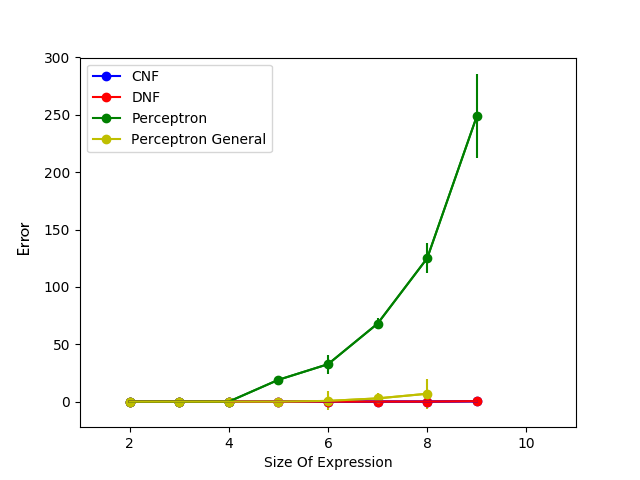
\includegraphics[width=\textwidth]{All-Peformance-Comparason.png}
    \caption{}
    \label{fig:peformance-comparason-all}
  \end{minipage}
  \hfill
\end{figure}

\begin{figure}[H]
  \centering
  \begin{minipage}[b]{0.8\textwidth}
    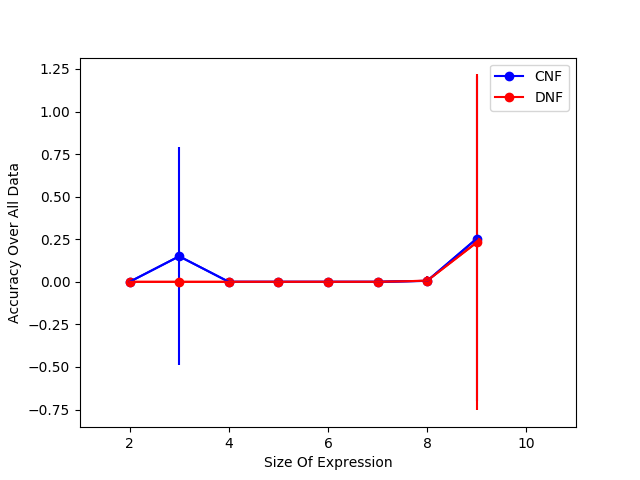
\includegraphics[width=\textwidth]{CNFvsDNF.png}
    \caption{}
    \label{fig:peformance-comparason-cnfdnf}
  \end{minipage}
  \hfill
\end{figure}

Figure  \ref{fig:peformance-comparason-all} shows that neither of the perceptron networks perform as well as the LNF Networks as $n$ increases. Figure  \ref{fig:peformance-comparason-cnfdnf} shows on average there are no statistically significant differences between the CNF or DNF networks. What is not present in  \ref{fig:peformance-comparason-cnfdnf} is that at $n = 9$ sometimes the CNF network far out performs the DNF and visa versa, theoretically both should be able to learn any boolean expression, this is something which will be investigated, as identified in the Chapter \ref{C:futureplan}. 

\section{LNF Network Generalization}
These networks are able to perform as well as standard perceptron networks but so far they have been getting the complete set of data, in practice this will almost never be the case. Standard ANN's are widely used because of their ability to generalize, for LNFN's to be useful they must also be able to generalize.

\begin{figure}[H]
	\centering
	\begin{minipage}[b]{0.8\textwidth}
		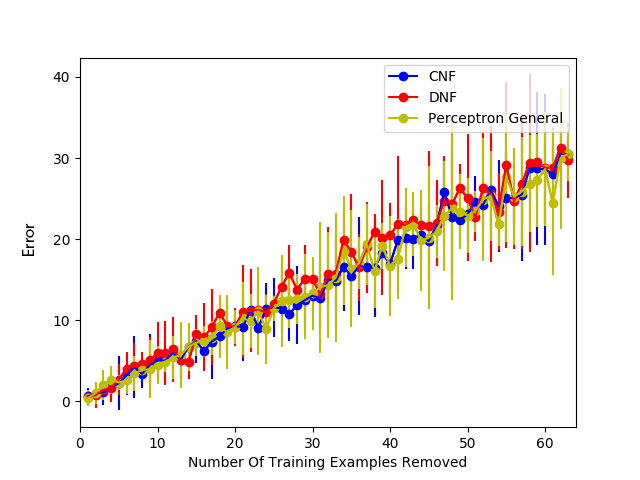
\includegraphics[width=\textwidth]{6-generalization.png}
		\caption{}
		\label{fig:generalization-peformance-6}
	\end{minipage}
	\hfill
\end{figure}

Figure \ref{fig:generalization-peformance-6} shows a comparison between the generalization ability of CNF, DNF and Perceptron networks. The graph shows the performance over all training data when successively removing elements from the training set. It demonstrates that the CNF and DNF networks generalize as well as the perceptron networks when the boolean formula has 6 inputs, this trend continues as n increases up to 9.

\section{LNF Network Rule Extraction}
The goal of this report is to learn rules which can be extracted from the network, consequently a method must be developed to extract the rules from LNF Network's. Take the weights of a trained LNFN, these weights can be converted back into $\epsilon_i$'s by apply the sigmoid function to each $w_i$.\\

As $\epsilon_i \rightarrow 0$ then $x_i$ becomes relevant and as $\epsilon_i \rightarrow 1$ then $x_i$ becomes irrelevant. If the network has learnt the correct DNF or CNF representation the for every neuron if input $i$ is relevant then $w_i \rightarrow -\infty$ and therefore $\epsilon_i \rightarrow 0$, otherwise $x_i$ is irrelevant and  $w_i \rightarrow \infty$ meaning $\epsilon_i \rightarrow 1$.\\

Consequently in $\epsilon$ form the weights of the LNFN are almost binary (i.e. very close to 0 or 1) and rules can be easily extracted as a boolean formula. Many clauses in the extracted expression contain redundant terms, i.e. clauses that are a tautology or a duplicate of another, filtering these out is not an expensive operation.\\

When training an LNFN over the entire truth table for a boolean expression, when a low error is achieved it is possible to extract boolean formula from the network which gets can generate the original truth table. This is a necessary first step but a more important question is, can formula still be extracted from the network when the LNFN is not trained with the entire truth table? If it can then what does this formula represent?
